\documentclass{article}

\usepackage{cite}
\usepackage[square, comma, numbers, sort&compress]{natbib}
\usepackage{wrapfig}
\usepackage[utf8]{inputenc}
\usepackage[T1]{fontenc}
\usepackage{lmodern}
\usepackage{amsfonts}
\usepackage{amsmath}
\usepackage{graphicx}
\usepackage{booktabs}
\usepackage{placeins}
% \usepackage{pdfpages}
\usepackage{caption}
\usepackage{multirow}
\usepackage{hhline}
\usepackage{capt-of}
\usepackage{array}
\usepackage{subcaption}
\usepackage{here}
\usepackage[labelfont=bf, format=plain, font=it]{caption}
\usepackage[german]{babel}


\begin{document}






\section{Wechselwirkung von Teilchen mit Materie}
\graphicspath{{bilder/1-1/}}
	\subsection{Wechselwirkung von geladenen Teilchen}
		\FloatBarrier

Nur die elektromagnetische Wechselwirkung ist von Bedeutung. Folgende Reaktionen führen zu einem
Energieverlust von geladenen Teilchen in Materie:

\begin{itemize}
  \item Ionisation der Atome im Detektormaterial
  \item Anregung der Atome im Detektormaterial
  \item Bremsstrahlung (relevant für Elektronen/Positronen)
  \item \v{C}erenkov-Strahlung
  \item Übergangsstrahlung
\end{itemize}

% \[-\left(\frac{dE}{dx}\right)_{\text{tot}} = -\left(\frac{dE}{dx}\right)_{\text{coll}}
% -\left(\frac{dE}{dx}\right)_{\text{rad}} -\left(\frac{dE}{dx}\right)_{\text{pair}}
% -\left(\frac{dE}{dx}\right)_{\text{photo}} -\left(\frac{dE}{dx}\right)_{\text{compt}}
% -\left(\frac{dE}{dx}\right)_{\text{kal}}-\ldots\]
 
 Beispiel: Gesamte Energieverlustrate $-\frac{dE}{dx}$ für Myonen in Kupfer (s. Abb.
 \ref{myonenInKupfer)}). Der Großteil wird durch die Bethe-Bloch-Formel beschrieben (Herleitung
 erfolgt im nächsten Kapitel).
Unterschiedliche Energie der Projektile führt über unterschiedliche Wechselwirkung zum
Energieverlust.

\begin{align*}
-\left(\frac{\mathrm{d}E}{\mathrm{d}x}\right)_{\text{tot}} &= -\left(\frac{\mathrm{d}E}{\mathrm{d}x}\right)_{\text{coll}}
-\left(\frac{\mathrm{d}E}{\mathrm{d}x}\right)_{\text{rad}} -\left(\frac{\mathrm{d}E}{\mathrm{d}x}\right)_{\text{pair}}
-\left(\frac{\mathrm{d}E}{\mathrm{d}x}\right)_{\text{photo}} -\left(\frac{\mathrm{d}E}{\mathrm{d}x}\right)_{\text{compt}} \\
&\hspace{4mm} -\left(\frac{\mathrm{d}E}{\mathrm{d}x}\right)_{\text{kal}}-\ldots
\end{align*}
 
\begin{figure}
	\centering
	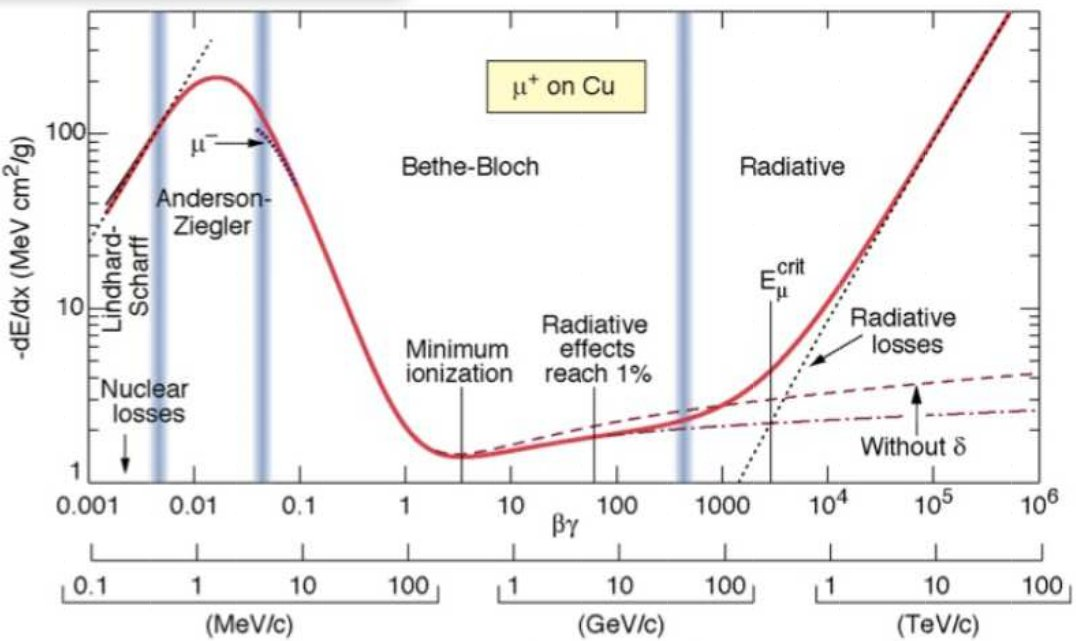
\includegraphics[width=0.5\textwidth]{bethebloch.jpg}
 	\caption{Energieverlust von Myonen in Kupfer}
 	\label{myonenInKupfer}
\end{figure}

\begin{figure}
	\centering
	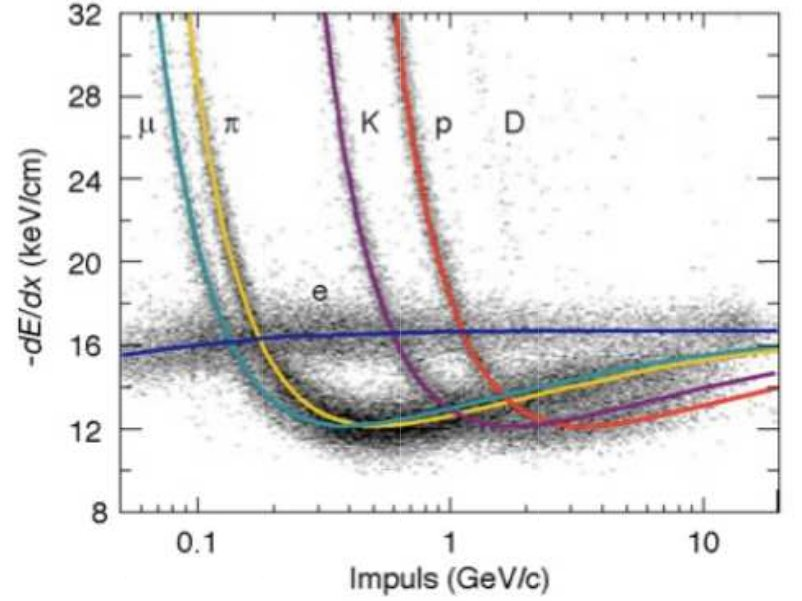
\includegraphics[width=0.5\textwidth]{bethebloch2.jpg}
	\caption{$\frac{dE}{dx}$-Kurven für verschiedene Teilchen (gemessen in der
	PEP4/9-TPC)}
	\label{}
\end{figure}
 
 Beachte: $\frac{dE}{dx}$ für "`schwere"' Teilchen (z.B. $\alpha$) wird in diesem Impulsbereich gut
 durch die Bethe-Bloch-Formel beschrieben. Der Energieverlust durch Ionisation und Anregung von
 Targetelektronen dominiert. $\frac{dE}{dx}$ für Elektronen/Positronen folgt jedoch nicht der
 Bethe-Bloch-Formel!
 
 \FloatBarrier
			\subsubsection{Bethe-Bloch-Formel}
				Zur klassischen Herleitung der Bethe-Bloch-Formel betrachten wir den Energieverlust $\frac{dE}{dx}$
eines schweren (d.h. $m>>m_e$), geladenen Teilchens durch Streuung an einem Hüllenelektron eines
Targetatoms.
\\
Dabei gelten folgende Annahmen:
\begin{itemize}
  \item das Hüllenelektron ist in Ruhe (Vernachlässigung der Bahnbewegung und des Rückstoßes),
  \item der Energieübertrag ist sehr viel größer als die Bindungsenergie eines Hüllenelektrons.
\end{itemize}


{\Huge ZEICHNUNG}

Der Impulsübertrag ist das Zeitintegral der durch das elektrische Feld des Projektils auf das
Target einwirkenden Kraft. Für die longitudinalen bzw. transversalen Komponenten des E-Feldes gilt

\[E_l(-x)=-E_l(x)~~~~~~~~~~~~~~~~~~~E_t(-x)=E_t(x)\]

d.h. nur der Transversalanteil ist wichtig, die longitudinalen Komponenten im Impulsübertrag heben
sich auf. Es gilt daher

\[\Delta p= \int_{-\infty}^{\infty}F\cdot dt = \int_{-\infty}^{\infty}eE_t\cdot dt =
e\int_{-\infty}^{\infty}E_t\frac{dt}{dx}\cdot dx
=e\int_{-\infty}^{\infty}E_t\frac{1}{v}\cdot dx
=\frac{e}{v}\int_{-\infty}^{\infty}E_t\cdot dx\]

Mit Gauß $\int_{-\infty}^{\infty}E_t2\pi bdx=4\pi ze$ folgt

\[\Delta p = \frac{2ze^2}{vb}\]

und somit für den Energieübertrag

\[\Delta E=\frac{\Delta p^2}{2m_e}=\frac{2z^2e^4}{m_ev^2b^2} .\]

Eine Elektronendichte von $n_e$ ergibt daher einen Energieverlust von 

\[-dE(b)=\Delta E(b)n_edv=\frac{2z^2e^4}{m_ev^2b^2}n_e2\pi b db dx\]

Nach der Integration von $b_min$ bis $b_max$ erhält man daraus:

\[-\left(\frac{dE}{dx}\right)=\frac{4\pi z^2
e^4}{m_ev^2}n_e\text{ln}\left(\frac{b_{\text{max}}}{b_{\text{min}}}\right)\]

Nun müssen nur noch $b_{\text{min}}$ bis $b_{\text{max}}$ abgeschätzt werden. $b_{\text{min}}$ wird über das
kinematische Limit abgeschätzt: Eine frontale Kollision liefert den maximalen Energieübertrag

\[\Delta E_{\text{max}}=\frac{1}{2}m_e(2v)^2\gamma^2.\]

Mit der oben abgeleiteten Beziehung

\[\Delta E(b)=\frac{2z^2e^4}{m_ev^2b^2}\overset{!}{=}\Delta E_{\text{max}}\]

ergibt sich daraus:

\[b_{\text{min}}=\frac{ze^2}{\gamma m_e v^2}.\]

Die Abschätzung von $b_{\text{max}}$ folgt aus der "`adiabatischen Invarianz"': Die Targetelektronen
sind in Atomen gebunden und "`umkreisen"' die Atomkerne mit einer mittleren Orbitalfrequenz
$\overline{\nu}$. Damit ein Energieübertrag stattfindet, muss die Zeitdauer der Störung, $\Delta t$,
kürzer sein als die Periodendauer $\tau$:

\[\Delta t=\frac{b}{\gamma v} \le \tau =\frac{1}{\overline{\nu}}\]

Daraus folgt

\[b_{\text{max}}=\frac{\gamma v}{\overline{\nu}}.\]

Jetzt führen wir noch eine Größe for die Elektronen-Dichte des Target-Materials ein:

\[n_e=N_A\cdot \rho\cdot \frac{Z}{A}\]

mit der Avogadrozahl $N_A$, der Targetdichte $\rho$, der Ordnungszahl $Z$ und der Massenzahl $A$.
Einsetzen der Grenzen für den Stoßparameter in die Formel und Substitution von $n_e$ führt zu

\[-\left(\frac{dE}{dx}\right)_{\text{coll}} = \frac{4\pi z^2e^4}{m_ev^2}N_A\cdot \rho
\frac{Z}{A}\cdot\text{ln}\left(\frac{\gamma^2 m_e v^3}{2e^2\overline{\nu}}\right), \]

was der klassischen Formel von Bohr entspricht. Diese beschreibt den Energieverlust für schwere
Teilchen (Protonen, $\alpha$-Teilchen,\ldots) durch Anregung und Ionisation. Für leichte Teilchen
müssen Quanteneffekte berücksichtigt werden.
\\
Die quantenmechanische Rechnung führt zur Bethe-Bloch(-Sternheimer)-Formel:

\[-\left(\frac{dE}{dx}\right)_{\text{coll}} = 2\pi N_A r_e^2 m_e c^2 \rho \frac{Z}{A}
\frac{z^2}{\beta^2}\left[ \text{ln} \left( \frac{2m_e c^2 \gamma^2 \beta^2 W_{\text{max}}}{I^2}
\right) -2\beta^2 -\delta -2\frac{c}{z} \right]\]

mit 

\[\beta =
\frac{v}{c},~~~~~~~~~~~~\gamma=\frac{1}{\sqrt{1-\beta^2}}~~~~~~~~~~~~
r_e=\frac{1}{4\pi\epsilon_0}\cdot\frac{e^2}{m_e c^2}\]

sowie
\begin{description}
\item[$z$]Ladung des einfallenden Teilchens
\item[$Z, A$] Ordnungs- und Massenzahl des Targets
\item[$\rho$] Targetdichte
\item[$N_A$] Avogradozahl
\item[$I$] mittleres Ionisationspotential (Materialkonstante des Targets)
\item[$W_{\text{max}}$] max. Energieübertrag in einer Einzelkollision
\item[$\delta$] Dichtekorrektur (Polarisationseffekt, $\delta \approx 2\text{ln}(\gamma)+K$)
\item[$c$] Schalenkorrektur (wichtig für kleine Projektilgeschwindigkeiten)
\end{description}


Anmerkungen zur Bethe-Bloch-Formel:
\begin{itemize}
  \item sie beschreibt den Energieverlust sehr gut im Bereich $0,1 < \gamma\beta < 100$;
  \item es gibt drei Bereiche:
  			\begin{itemize}
  			  \item bei niedrigen Energien gibt es einen Abfall bis zu einem Minimum (bei $\gamma\beta$
  			  ca. 3-3,5), Teilchen an diesem Punkt sind minimal ionisierende Teilchen;
  			  \item danach beginnt ein logarithmischer Anstieg mit zunehmender Teilchenenergie, der
  			  sogenannte "`relativistische Anstieg"';
  			  \item bei hohen Energien wird das Fermi-Plateau erreicht: durch Polarisationseffekte erreicht
  			  der Energieverlust  einen Sättigungswert (Dichtekorrektur);
  			  \end{itemize}
  \item beim Energieverlust handelt es sich um einen statistischen Vorgang.
\end{itemize}

Die Bethe-Bloch-Formel beschreibt den mittleren Energieverlust durch Ionisation und Anregung. Sie
gilt für alle geladenen Teilchen außer Elektronen und Positronen. Für diese muss die Gleichheit der
Massen und die Ununterscheidbarkeit der Stoßpartner berücksichtigt werden. Unsere Ableitung
unterscheidet sich von der Bethe-Bloch-Formel numerisch durch einen Faktor 2, was durch eine
mangelhafte Berücksichtigung von Fernstößen zustande kommt. Für die quantenmechanische Beschreibung
des Energieverlustes gibt es verschiedene Varianten der $\frac{dE}{dx}$-Formel, was an der
unterschiedlichen Parametrisierung der Fernstöße, d.h. jenes Energieverlustes, bei dem die Bindung
der Elektronen in den Atomhüllen nicht vernachlässigbar ist.
\\
Meist wird der Energieverlust pro Wegstrecke $\frac{1}{\rho}\frac{dE}{dx}$ angegeben, wobei $\rho$
die Dichte in $\frac{\text{g}}{\text{cm}^3}$ ist. $\frac{1}{\rho}\frac{dE}{dx}$ ist für ein MIP nur
schwach vom Absorbermaterial abhängig und beträgt ca. 

\[2 \text{MeV}\frac{\text{cm}^2}{\text{g}}.\]
			\subsubsection{Landau-Verteilung}
				\FloatBarrier
Wie kann die Energieverteilung des Energieverlustes für ein gegebenes "`$\beta\cdot\gamma$"' beschrieben
werden? Der Energieverlust ist ein statistischer Prozess mit einer asymmetrischen
Verteilungsfunktion, da Kollisionen mit kleinem Energieübertrag wahrscheinlicher sind als solche
mit großen Energieübetrag.

\begin{figure}
	\centering
	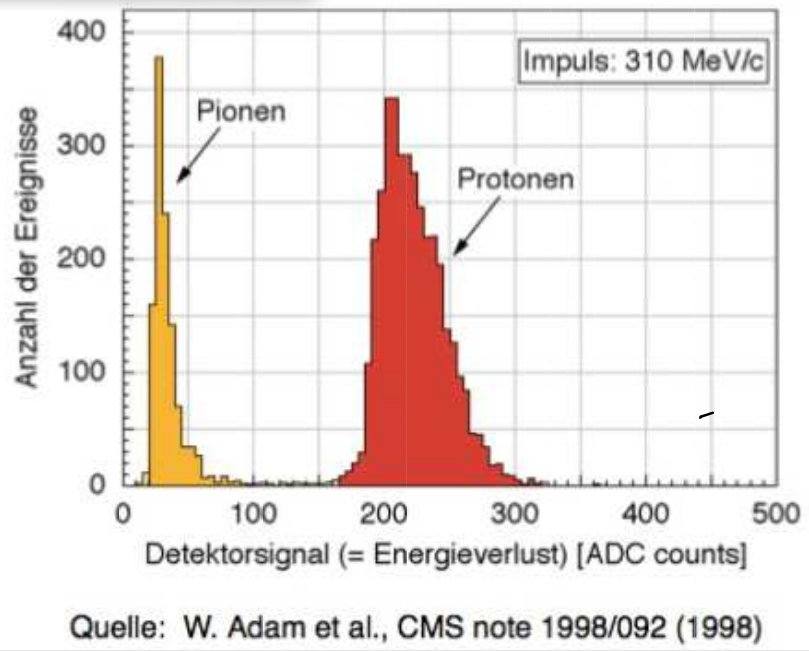
\includegraphics[width=0.5\textwidth]{landau.jpg}
	\caption{Die Energieverteilung des Energieverlustes ist eine Landau-Verteilung.}
	\label{}
\end{figure}

Der Ausläufer bei hohen Energieüberträgen kommt von (selten auftretenden) Kollisionen mit kleinen
Stoßparametern, wobei Elektronen mit großen Ener\-gien (keV), sogenannte $\delta$-Elektronen,
freigesetzt werden. Die Asymmetrie kommt daher, dass der mittlere Energieverlust höher
ist als der wahrscheinlichste Energieverlust.
\\
Bei dünnen Absorbern wird der Energieverlust durch eine Landau-Verteilung beschrieben, bei dicken
Absorbern geht diese über in eine Gauß-Verteilung.

\FloatBarrier
			\subsubsection{Bragg-Kurve}
				Wie tief dringen Teilchen in das Detektormaterial ein? Man kann für jede
Projektil/Target-Kombination nur eine mittlere Eindringiefe angeben. Der Energieverlust eines
Projektils in Anhängigkeit von der Eindringtiefe wird durch die Bragg-Kurve beschrieben. Mit
Eindringen in die Materie wird das Projektil langsamer, der Energieverlust steigt an
(Bethe-Bloch). Die Reichweite $R$ enthält man aus der Integration des Energieverlustes entlang des
Weges, wobei $\frac{dE}{dx}$ hierbei eine Funktion von $E$ ist. Bei ionisierender Strahlung kommt es
am Ende der Reichweite wegen $\frac{1}{\beta^2}$-Verhalten zu einer besonders hohen Dichte der
deponierten Energie.

\[dE= \frac{dE}{dx}(E)dx~~~~~~~~~~\Rightarrow~~~~~~~~~~dx
=\frac{dE}{dE/dx}~~~~~~~~~~\Rightarrow~~~~~~~~~~ R=\int_{E_c}^{M} \frac{dE}{dE/dx}  \]

Der größte Ionisationsverlust findet nahe am Ende der Spur statt (Bragg-Peak).



% Absorptionsprozesse (mit $dN=8\mu dx$) führen zu einem exponentiellen Abfall der Teilchenzahl.

% \begin{figure}
% \begin{minipage}{0.45\textwidth}
% 
% \end{minipage}
% \begin{minipage}{0.45\textwidth}
% 
% \end{minipage}
% \caption{bla}
% \end{figure} 

\begin{figure}[htbp]
	\begin{minipage}[b]{0.5\textwidth}
		\begin{figure}[H]
		\centering
		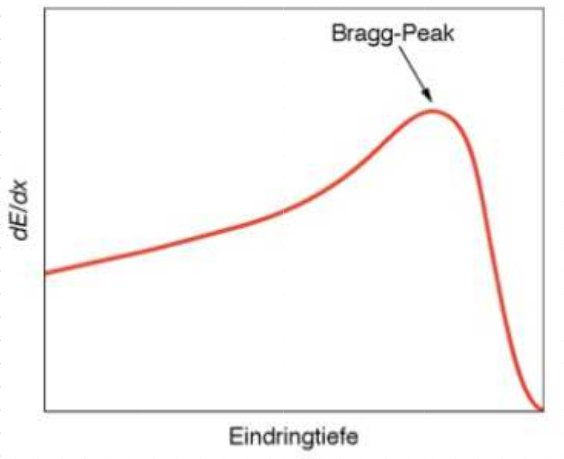
\includegraphics[width=\textwidth]{bragg.jpg}
		\end{figure}
	\end{minipage}
	\hfill
	\begin{minipage}[b]{0.5\textwidth}
		\begin{figure}[H]
		\centering
		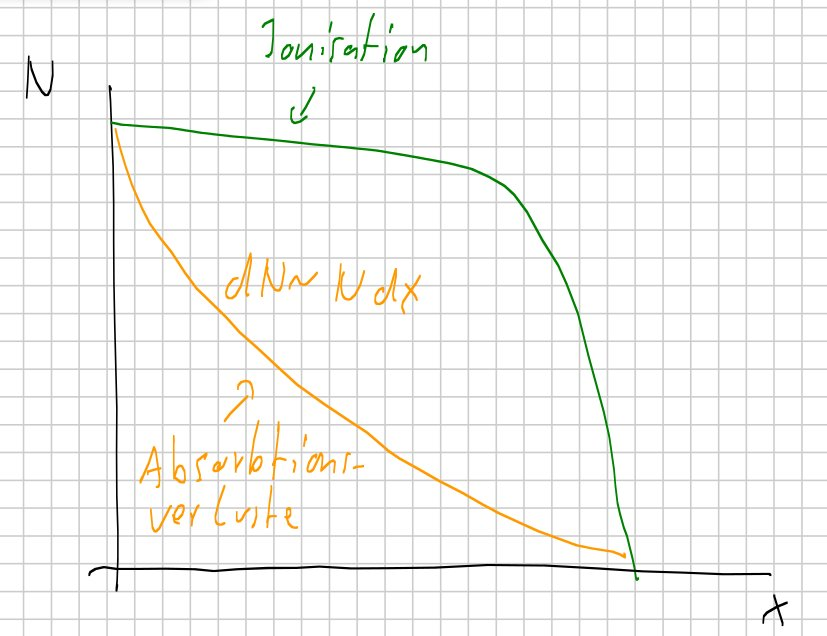
\includegraphics[width=\textwidth]{expabfall.jpg}
		\end{figure}
	\end{minipage}
	\caption{b}
	\label{rekristall} 
\end{figure}




\end{document}